\documentclass[letterpaper,10pt]{article}
\usepackage[top=2cm, bottom=1.5cm, left=1cm, right=1cm]{geometry}
\usepackage{amsmath, amssymb, amsthm,graphicx}
\usepackage{fancyhdr}
\pagestyle{fancy}

\lhead{\today}
\chead{Multivariate Stats Exam 2}
\rhead{Justin Hood}

\newcommand{\Z}{\mathbb{Z}}
\newcommand{\Q}{\mathbb{Q}}
\newcommand{\R}{\mathbb{R}}
\newcommand{\C}{\mathbb{C}}
\newtheorem{lem}{Lemma}

\begin{document}
\begin{enumerate}
\item We first consider the quality improvement data,
\begin{center}
\begin{tabular}{|r|rrrrrrrrrrrr|}
\hline
Level/Obs & 1 & 2 & 3 & 4 & 5 & 6 & 7 & 8 & 9 & 10 & 11 & 12\\\hline
1 & 7.6 & 8.2 & 6.8 & 5.8 & 6.9 & 6.6 & 6.3 & 7.7 & 6.0 &&& \\\hline
2 & 6.7 & 8.1 & 9.4 & 8.6 & 7.8 & 7.7 & 8.9 & 7.9 & 8.3 & 8.7 & 7.1 & 8.4\\\hline
3 & 8.5 & 9.7 & 10.1 & 7.8 & 9.6 & 9.5 &&&&&&\\\hline
\end{tabular}
\end{center}
Breaking the data down into a digestible form, we obtain the following plot,
\begin{center}
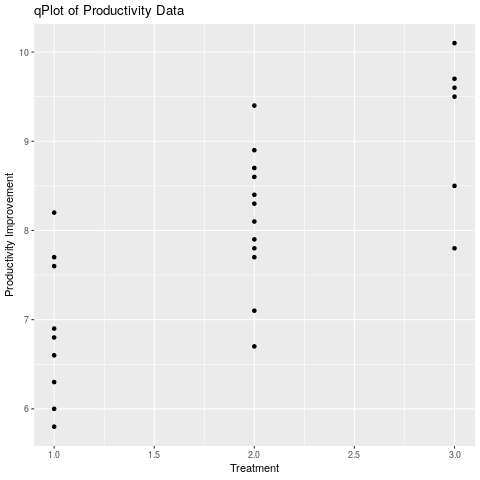
\includegraphics[scale=.75]{prodq.png}
\end{center}
From a purely observational perspectivem we see that the different treatments have fairly unique values of improvement. As such, we expect that the level factors will be significant in the analysis.\\
Then, using $R$, we perform the ANOVA analysis. By treating the levels of the R\& D development as factors in $R$, we obtain the following ANOVA table,
\begin{center}
\begin{tabular}{|r|rrrrr|}
\hline
& Df & Sum Sq & Mean Sq & F & p-value\\\hline
Level & 2 & 20.12 & 10.06 & 15.72 & $4.33\times 10^{-5}$\\
Residuals & 24 & 15.36 & 0.64 &&\\\hline
\end{tabular}
\end{center}
For our analysis, we will test the following hypotheses,
\begin{align*}
H_0:\ & \mu_1=\mu_2=\mu_3\\
H_A:\ & \exists \mu_i\neq \mu_j\ i,j\in \{1,2,3\}
\end{align*}
We test this hypothesis with the $F$ statistic, $F=15.72$ from before. With associated $p$-value, $p=.0000433$. Using $\alpha=0.05$, we will reject the null hypothesis, and conclude that there is a difference in the means of the different treatments. As such, we will create 1-$\alpha$\% confidence intervals comparing the means for further analysis. Using $R$, we obtain the Tukey intervals,
\begin{center}
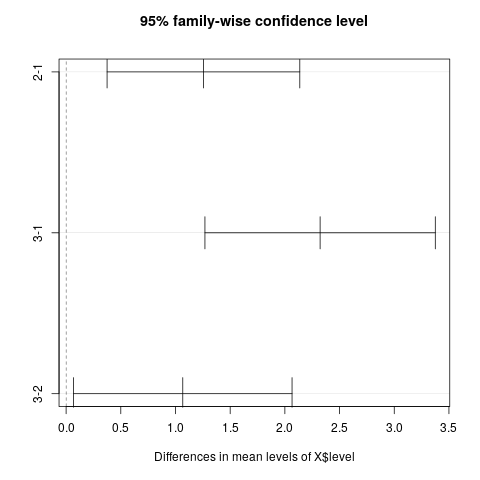
\includegraphics[scale=.75]{prodtukey.png}
\end{center}
Here, we see that none of the different treatment pairs contains $0$ within their CI. As such, we further confirm our suspicions that their means are different. Looking further at the data, we can compute the following,
\begin{align*}
\mu_1 &= 6.97778\\
\mu_2 &= 8.13333\\
\mu_3 &= 9.2
\end{align*}
Looking again at the intervals, we see that the centers are precicely located at the difference in mean values, and that based on this, we obtain the following relationship,
\[\mu_3>\mu_2>\mu_1\]
While we may not make any rigorous statistical statements about the relationship, we can infer that the third level of treatment appears to be related to the largest increase in productivity. Assuming that the treatments are Low-Medium-High in terms of R\& D expenditure, we think that the high spending is potentially correlated to higher productivity improvements. 
\item Next, we consider the sheet metal data. To begin, we consider the first thirty data points. We are given that the process is stable for these points, and as such, we shall construct our $\bar{x}$ and $S$ matrices using these points. Using $R$, we obtain the following,
\begin{align*}
\bar{x} &= \begin{bmatrix}
-0.50633333 \\ -0.20700000\\ -0.06200000\\ -0.03166667\\  0.69800000\\ -0.06500000
\end{bmatrix}\\
S &= \begin{bmatrix}
0.062603333 & 0.0615851724 & 0.047383448 & 0.0082821839 & 0.01973862 & 0.003139655\\
0.061585172 & 0.0924493103 & 0.026771724 & -0.0008431034 & 0.02276483 & 0.015491379\\
0.047383448 & 0.0267717241 & 0.144616552 & 0.0078448276 & 0.02109931 & -0.004906897\\
0.008282184 & -0.0008431034 & 0.007844828 & 0.1086488506 & 0.02207241 & 0.006556897\\
0.019738621 & 0.0227648276 & 0.021099310 & 0.0220724138 & 0.34284414 & 0.014582759\\
0.003139655 & 0.0154913793 & -0.004906897 & 0.0065568966 & 0.01458276 & 0.036605172
\end{bmatrix}
\end{align*}
Constructing a $T^2$ chart on this data, we compute,
\[d_i=(X_i-\bar{x})S(X_i-\bar{x})\]
For the first thirty data points, we obtain the plot,
\begin{center}
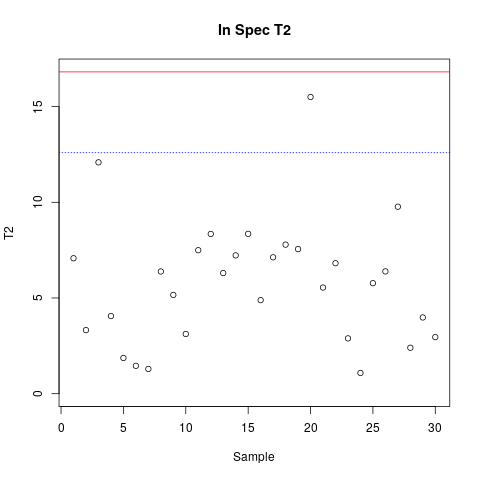
\includegraphics[scale=.75]{inspec.png}
\end{center}
Here, we have the blue line for the $95\%$ level, and the red line for the $99\%$ level. Here, we see that all of the data points are within the limits as noted before. Here, the level cutoffs are computed as,
\[UCL_{95}=\chi^2_p(.05)=12.59,\ UCL_{99}=\chi^2_p(.01)=16.81\]
with $p=6$, from the number of variables. Next, we extend this computation to all fifty data points, using the previously computed $\bar{x}$ and $S$. The resultant plot is,
\begin{center}
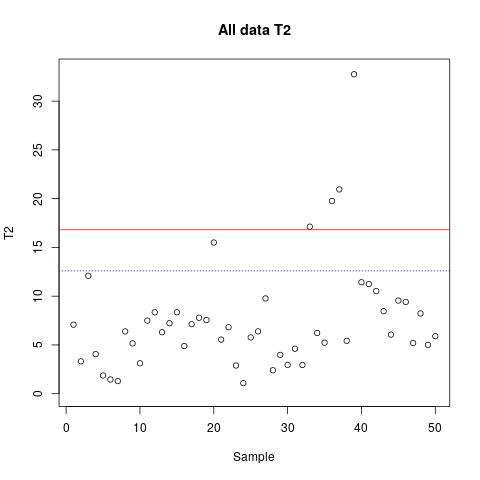
\includegraphics[scale=.75]{outspec.png}
\end{center}
We see that there appears to be 4 points that are outside of spec at the $99\%$ level. These points are,
\[\{33,\ 36,\ 37,\ 39\}\]
To test which of the locations is cause for concern, we construct $99\%$ confidence ellipses comparing the different variables. Plotting in $R$, we see that when comparing $x_1$ and $x_2$, and $x_1$ and $x_6$. The resultant plots are,
\begin{center}
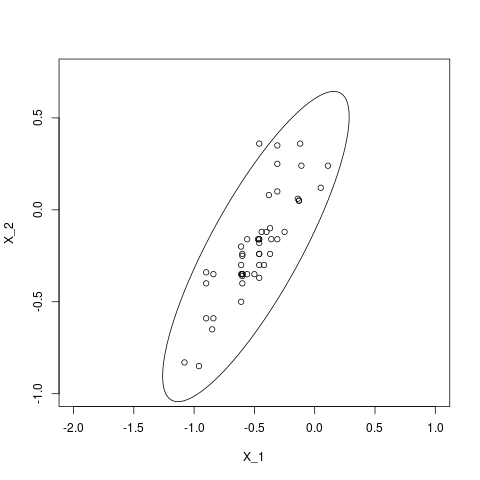
\includegraphics[scale=.7]{12.png}
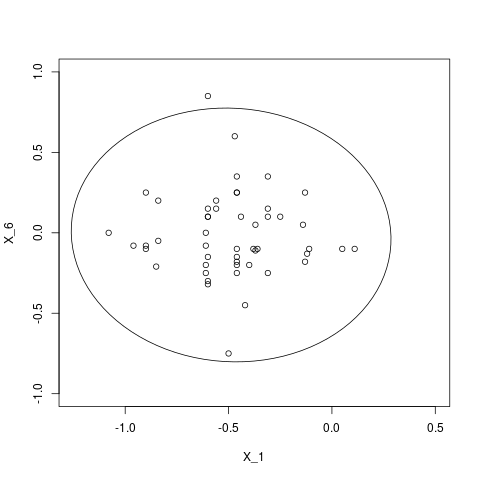
\includegraphics[scale=.7]{16.png}
\end{center}
Because these are the only plots with outliers, we conclude that $x_2$ and $x_6$ are variables with potential causes for concern.\\
Noting now that these measurements are deviations from a target value, we know that the zero vector is the ideal situation. So, we test the following,
\begin{align*}
H_0:\ & \mu=\textbf{0}\\
H_A:\ & \mu\neq\textbf{0}
\end{align*}
Setting $\alpha=.05$, we compute the test statistic,
\[T^2=n(\bar{x}-\mu)'S^{-1}(\bar{x}-\mu)=n(\bar{x})'S^{-1}(\bar{x})=374.7227\]
and our critical value,
\[T^*=\frac{p(n-1)}{n-p}F(\alpha)_{p,n-p}=18.18437\]
We see that $T^2>T^*$, and as such, we shall reject our null hypothesis in favor of the alternative, that at least one mean is not equal to zero. Based on our analysis, further investigation into locations 2 and 6 is a good potential start.
\item We now consider the BHO data. This data contains the percentage of discharges from mental health institutions that had a refill on the relevant prescription drugs perscribed, (Mood Stabilizers, Psychotropics, and Antipsychotics). To begin, we import the data with the given $R$ commands, and look at histograms of the relevant data columns. These plots follow,
\begin{center}
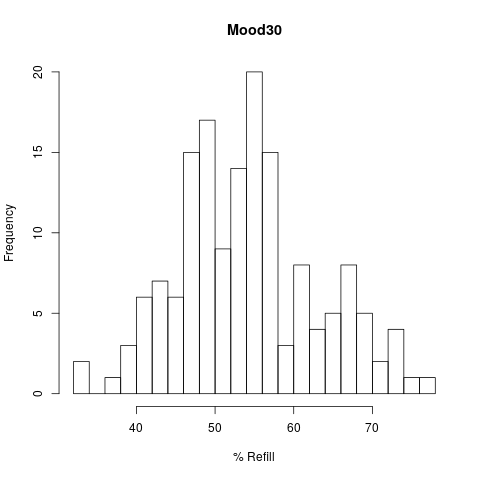
\includegraphics[scale=.33]{moodhist.png}
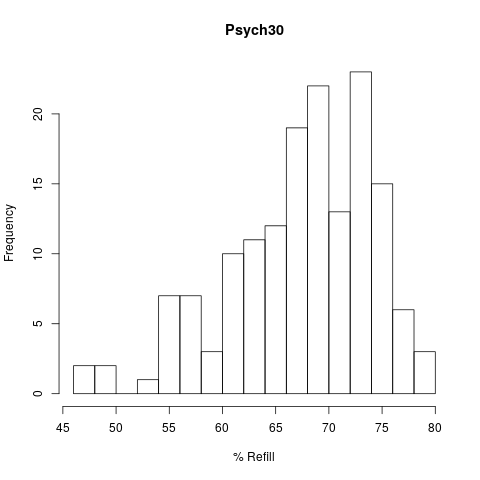
\includegraphics[scale=.33]{psychhist.png}
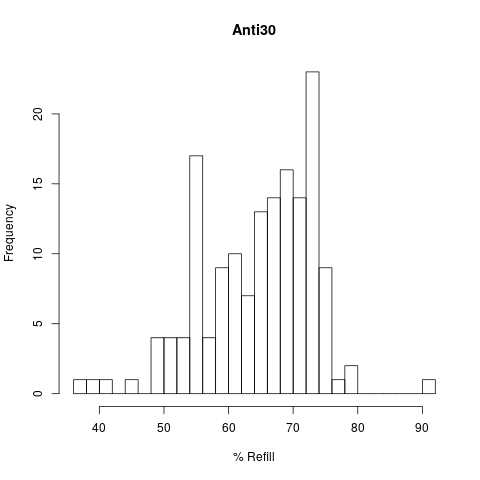
\includegraphics[scale=.33]{antihist.png}
\end{center}
We see from this data that the Mood stabilizers data appears to be quite normal, while the Psychotropic and Antipsychotics appear less normal. The latter two appear slightly skewed. This issue is again apparent from the $QQ$ plots for each individual data set. We shall look at these plots as well as the $r_Q$ statistic, from the text. For the Mood data,
\[r_Q=0.9917832\]
\begin{center}
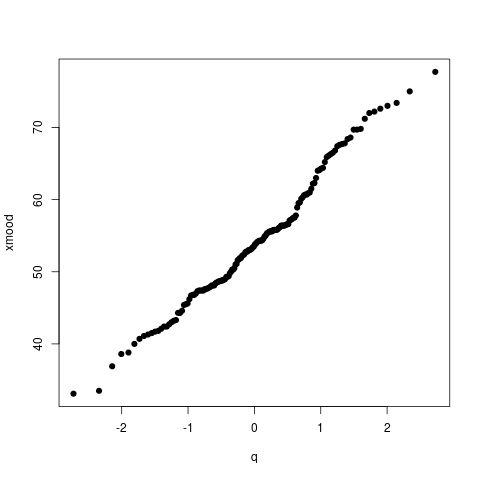
\includegraphics[scale=.5]{moodq.png}
\end{center}
For the Psycotropic data,
\[r_Q=0.9784581\]
\begin{center}
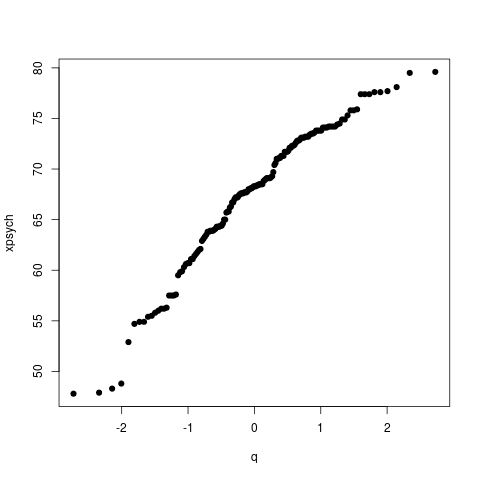
\includegraphics[scale=.5]{psychq.png}
\end{center}
For the Antipsychotic data,
\[r_Q=0.9790218\]
\begin{center}
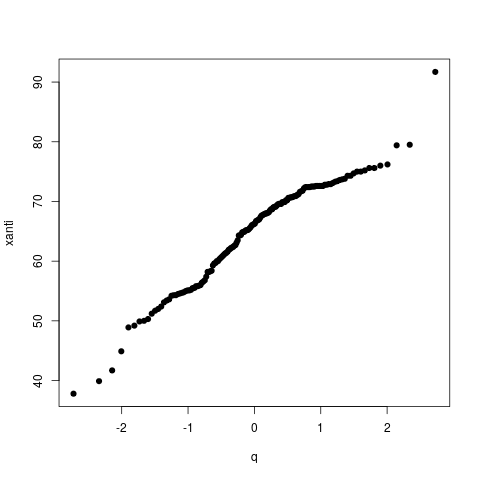
\includegraphics[scale=.5]{antiq.png}
\end{center}
From the text, we see that the cutoff for $r_Q^*\approx 0.9913$, so we see that only the mood data can clearly be called normal, as noted before. Let us now construct the Chi-square plot for the data to look for outliers.
\begin{center}
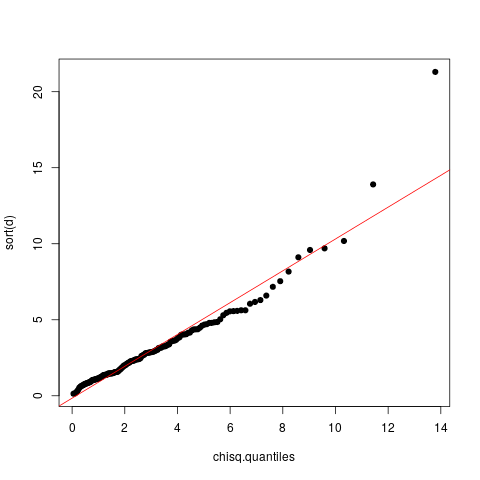
\includegraphics[scale=.8]{originalchi.png}
\end{center}
This plot is overlaid with the linear regression from the data. We see that the last point in the data is much further away from the rest. Looking into the data, we see that this point corresponds to an Antipsychotic value much higher than the norm. Looking further into this, we see that this point corresponds to $3.142141$ standard deviations above the mean. Because we cannot parse the data directly, we shall simply remove this point for brevity, and continue the analysis. We shall recompute the Chi-square plot without this data point,
\begin{center}
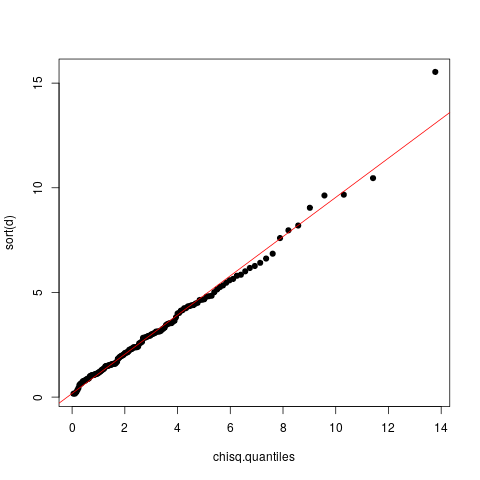
\includegraphics[scale=.8]{newchi.png}
\end{center}
Our new $QQ$ plots and $r_Q$ values are,
\begin{center}
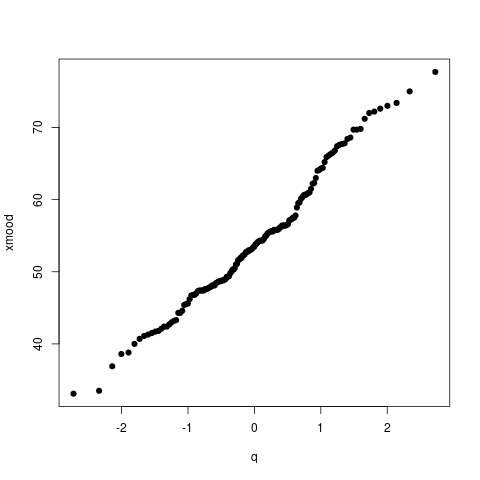
\includegraphics[scale=.33]{newmoodq.png}
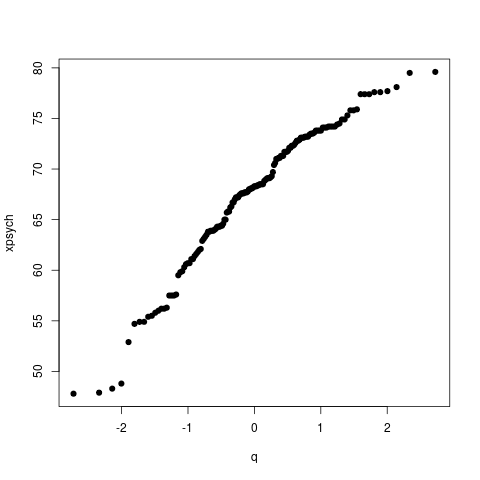
\includegraphics[scale=.33]{newpsychq.png}
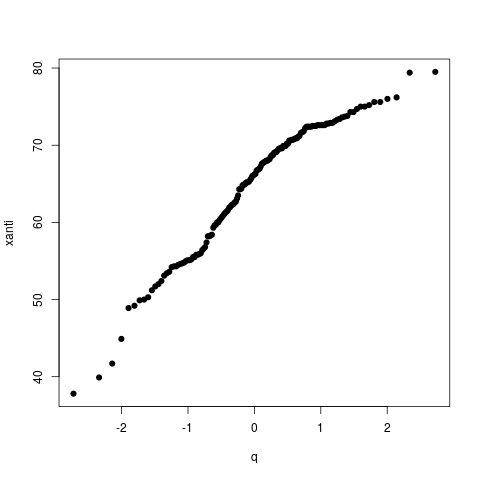
\includegraphics[scale=.33]{newantiq.png}
\end{center}
\begin{align*}
R_{Q_M} &= 0.9916236\\
R_{Q_P} &= 0.9786089\\
R_{Q_A} &= 0.9743146
\end{align*}
We see that the Psychotropic and Antipsychotic variables are still not quite normal. Because of this, we consider a power scaling on these two variables. We compute a range of possible values for the scaling according to the Box-Cox solution. The adjusted $QQ$ plots and appropriate scalings follow,
\begin{center}
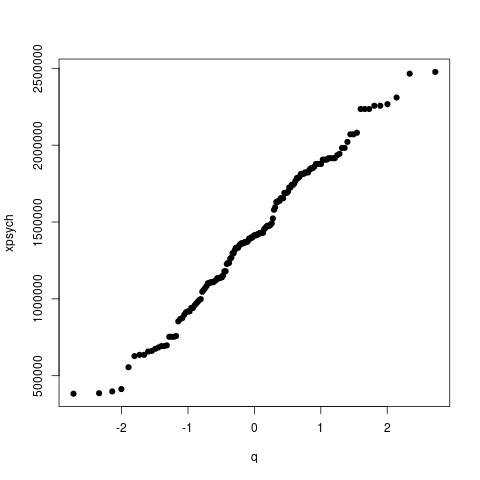
\includegraphics[scale=.5]{scalepq.png}
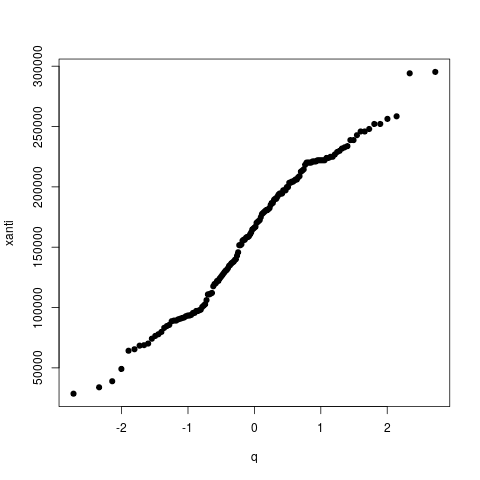
\includegraphics[scale=.5]{scaleaq.png}
\end{center}
\begin{align*}
\lambda_P &= 3.66\\
X_P &= \frac{X_P^{3.66}-1}{3.66}\\
\lambda_A &= 3.14\\
X_A &= \frac{X_A^{3.14}-1}{3.14}
\end{align*}
We see that this new scaling results in a value of $r_Q$ for Psychotropics that is above the cutoff for normalcy, and a value for Antipsychotics that is very close. We again construct the Chi-square plot,
\begin{center}
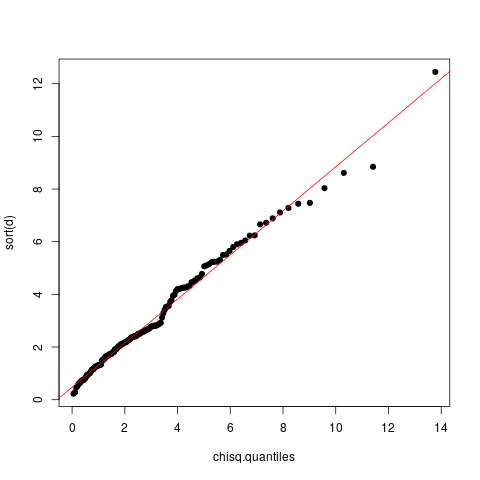
\includegraphics[scale=.75]{bestchi.png}
\end{center}
We see that this plot is quite linear, which backs up our analysis that the data is normal. As we have optimized all we can, we shall continue the analysis. So, we now perform a $T^2$ test on the new data,
\[X=\begin{bmatrix}
X_M & \frac{X_P^{3.66}-1}{3.66} & \frac{X_A^{3.14}-1}{3.14}
\end{bmatrix}\]
Our hypotheses are then,
\begin{align*}
H_0:\ & \mu=[75,\ 75,\ 75]\\
H_A:\ & \mu \neq [75,\ 75,\ 75]
\end{align*}
Because we have scaled the data, we find the adjusted $\mu$ to be,
\[\mu=[75,\ \frac{75^{3.66}-1}{3.66},\ \frac{75^{3.14}-1}{3.14}]=[75,\ 1991787.851,\ 245902.0541]\]
From this, we compute both $T^2$ and $T^*$ as,
\begin{align*}
T^2 &= 906.8405\\
T^* &= 8.097482
\end{align*}
Because $T^2>T^*$, we shall reject the null hypothesis, in favor of the alternative, that at least one of the means is not $75\%$. For further analysis, we look at the cleaned data, and see that our sample means are,
\[\mu=[54.103,\ 1411823,\ 161341]\]
Which, when we unscale the data, corresponds to a mean of,
\[\mu=[54.103,\ 68.269,\ 65.856]\]
Based on the fact that we are comparing to a mean of $75$, we see that our samples are much less on average than our test value. So, we would expect that at least one of the variables is significantly less. Looking at the means of the cleaned data, we would expect at least the Mood stabilizers data to be significantly less, but further analysis is required to say for sure.
\item Finally, we consider the City of Bloomington Indiana data. Using the provided $R$ code to import the data, we find that we have two columns of 57 data points in the form of (TTHM, HAA5). These columns refer to the content in $\mu g/L$ for trihalomethanes and Haloacedic acids respectively. To begin, we look at the histograms of the data,
\begin{center}
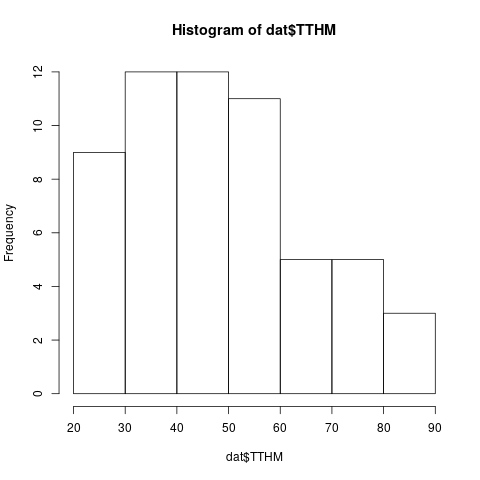
\includegraphics[scale=.5]{thist.png}
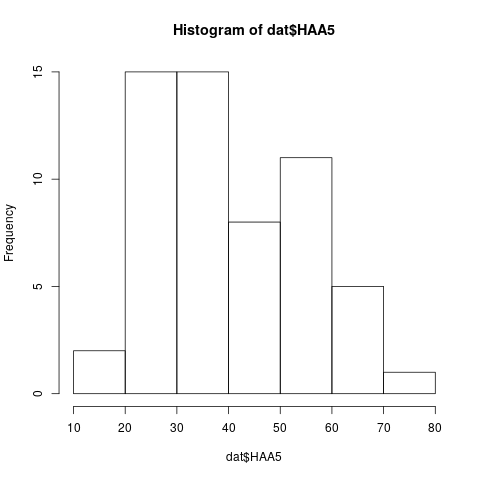
\includegraphics[scale=.5]{hhist.png}
\end{center}
We see that the data is roughly normal, so we proceed with further control chart analysis. First, we consider the $\bar{X}$ charts for each variable. We compute,
\begin{align*}
UCL &= \bar{\bar{x}}_i+3\sigma_i\\
LCL &= \bar{\bar{x}}_i-3\sigma_i
\end{align*}
as bounds on the data for testing control. Because our data is a measured quantity, we bound the lower limit by 0 for completeness, so we shall make the note,
\[LCL=\max(0,\ \bar{\bar{x}}_i-3\sigma_i)\]
Plotting,
\begin{center}
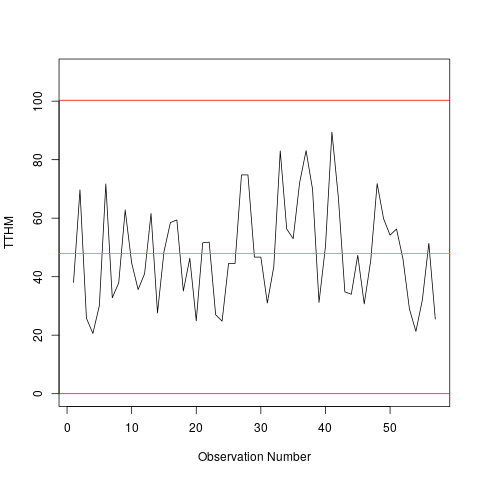
\includegraphics[scale=.5]{tthmxbar.png}
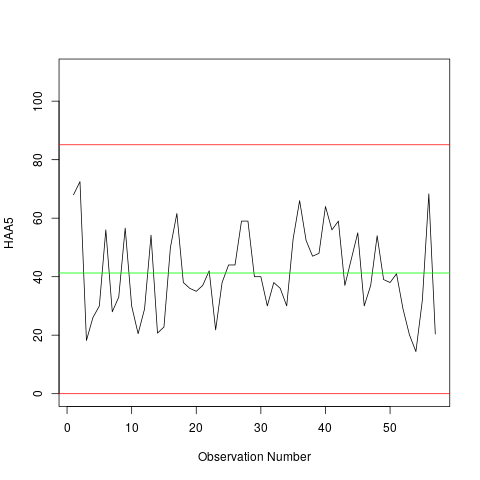
\includegraphics[scale=.5]{haa5xbar.png}
\end{center}
First, looking at the TTHM plot, we see that there is random variation around the mean, as well as no clear trends in the data, so we conclude that the variable is under control. For the HAA5 variable, we see that there is the same random varaition around the mean, and no clear trends, so this variable is also in control. \\
Next, we create an ellipse format chart of the data. Using $\alpha=0.01$, we construct the quality ellipse,
\[(x-\bar{x})'S^{-1}(x-\bar{x})\leq \chi_2^2(\alpha)\]
\begin{center}
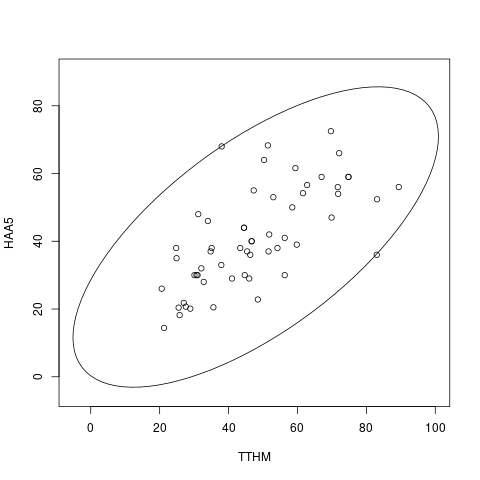
\includegraphics[scale=.75]{waterelip.png}
\end{center}
Looking at the data in this form, we see that there is one point at approximately $(85,\ 35)$. Further inspection of the data confirms the point to be, $(83.0,\ 36.0)$. This point is right on the boundary of the ellipse, so it is worth further exploration.\\
Next, we construct the $T^2$ chart for the data, as before. The plot follows, with the $95\%$ cutoff in blue, and the $99\%$ cutoff in red. 
\begin{center}
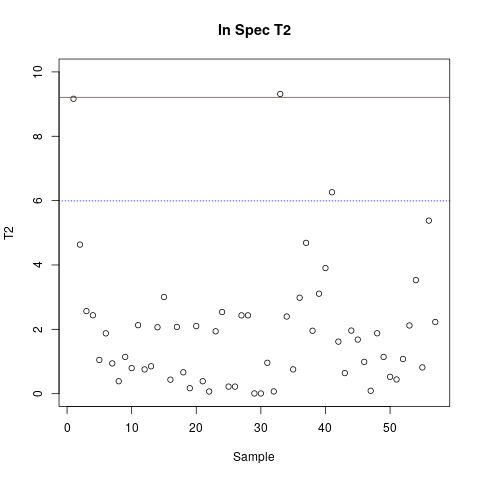
\includegraphics[scale=.75]{watert.png}
\end{center}
Similarly to the ellipse chart, we see that there is only the one point that is outide of the cutoff. So we again see that this point is worth further investigation. It is possible that there was a misread in the sampling process, or that an external event such as a water main break that caused an artificial inflation in the data. Finally, we perform a $T^2$ test on the data with hypotheses,
\begin{align*}
H_0:\ & \mu=[80,\ 60]\\
H_A:\ & \mu\neq [80,\ 60]
\end{align*}
Computing,
\begin{align*}
T^2 &= 192.8599\\
T^* &= 6.445077
\end{align*}
Given that $T^2>T^*$, we reject the null hypothesis in favor of the alternative, that the mean is not the maximum allowable level. Looking at the data means, we see that the sample has mean vector,
\[\mu=[47.87719,\ 41.25439]\]
Given that these values are less than the maximal allowable level, we see that at least one of these variables are less than the maximal allowable level. Further analysis is reqired to test whether the mean is less than the maximal vector.
\end{enumerate}
\end{document}
